Para revisar la diferencia en eficiencia entre distintas implementaciones de \textsc{trafico} sobre el algoritmo de Djikstra consideramos tres algoritmos para solucionar este problema. El primero, al que llamaremos \textit{heap}, utiliza un heap para guardar todas las aristas y luego ir sacando las candidatas. y puede extraer el mínimo en tiempo constante y cambiar una clave en un razonable $\Theta(log(n))$. La complejidad temporal de este algoritmo es $\Theta(mlogn)$\footnote{Ver diapositivas de la clase 7, AED3}. Una segunda implementacion, a la que llamaremos \textit{ingenua}, funciona de la misma manera pero implementa el heap de forma ingenua, con un arreglo de costos y otro de valores. Esto permite cambiar claves en tiempo constante, pero a cambio encontrar el mínimo se hace en $Theta(n)$. La complejidad resultante es $Theta(n^2)$\footnote{Ver diapositivas de la clase 7, AED3}. Finalmente usamos \textit{queue}, una implementacion que utiliza la cola de prioridad del \textit{prelude} de C$++$ y un arreglo \textit{marcados} que indica si un elemento ya pasó por el queue o no. En vez de agregar todos los nodos a la cola como los otros dos algoritmos, este los va colocando en a medida que aparecen en la lista de adyacencia de los nodos candidatos. El arreglo \textit{marcados} evita que se repitan nodos. Tiene complejidad espacial de $Theta(mlogn)$\footnote{Ver diapositivas de la clase práctica 12 sobre camino mínimo}.

Teóricamente, \textit{ingenuo} será más eficiente para instancias \textit{densas}, mientras que los otros dos resultan especialmente buenos para entradas \textit{ralas}. Sin embargo los tres algoritmos tienen distintos detalles de implementación que resultan interesantes de analizar empíricamente: Si bien \textit{ingenuo} es asintóticamente superior, realiza mucho trabajo de más al tener que recorrer la estructura entera cada vez para encontrar el mínimo. \textit{Queue} puede recorrer el mismo nodo varias veces si se ingresó a la cola en múltiples instancias, y además no tiene el costo de cambiar claves dentro del heap, pero como queue es una estructura de \textit{prelude} es probable que esté bien optimizada, en comparación con \textit{heap} que fue implementada "a mano".

Para ver empíricamente la diferencia en eficiencia entre estas tres implementaciones, realizamos una serie de evaluaciones respecto al tiempo de ejecución en función del tamaño de la entrada, primero para muestras aleatorias de tamaño $N = 15000$ $M = 15000 + 11247750 * k$ para cada $k$ natural  en el rango $1 \leq k \leq 10$, para cómo afecta la cantidad de aristas al tiempo de ejecución en cada algoritmo, luego con muestras de tamaño $N = 10000k$ para cada $k$ natural en el rango $1 \leq k \leq 10$, para observar el desempeño en grafos ralos. Y finalmente con muestras de tamaño $N = 1000000k$ para cada $k$ natural en el rango $1 \leq k \leq 10$, para comparar el desempeño en grafos ralos de \textit{heap} y \textit{queue}.

Realizamos cada evaluacion diez veces para reducir la variación de los resultados y tomamos el promedio aritmético. Para la segunda evaluación lo hicimos 100 veces, dado que los tiempos eran pequeños.

A su vez, controlamos los parámetros de la función de la siguiente forma. Elegimos $K = 0$, $S = 1$, $T = 2$, y definimos cada arista $x_i = (a_i, b_i, w_i)$, para todo $1 \leq  i \leq M$, $0 \leq w_i \leq 1000$ y $1 \leq a_i b_i \leq N$ aleatorios, tal que $a_i \neq b_i$ y $(a_i, b_i) \neq (a_j, b_j)$ para todo $1 \leq i, j \leq M e i \neq j$

Notar que ninguna de estas decisiones afecta a la complejidad de las implementaciones de Djikstra. En efecto, el valor de K solo es relevante luego de haber corrido Djikstra, y S y T aleatorios no deberían tener efecto sobre la complejidad asintóticamente.

\begin{figure}[!htbp]
    \subfloat{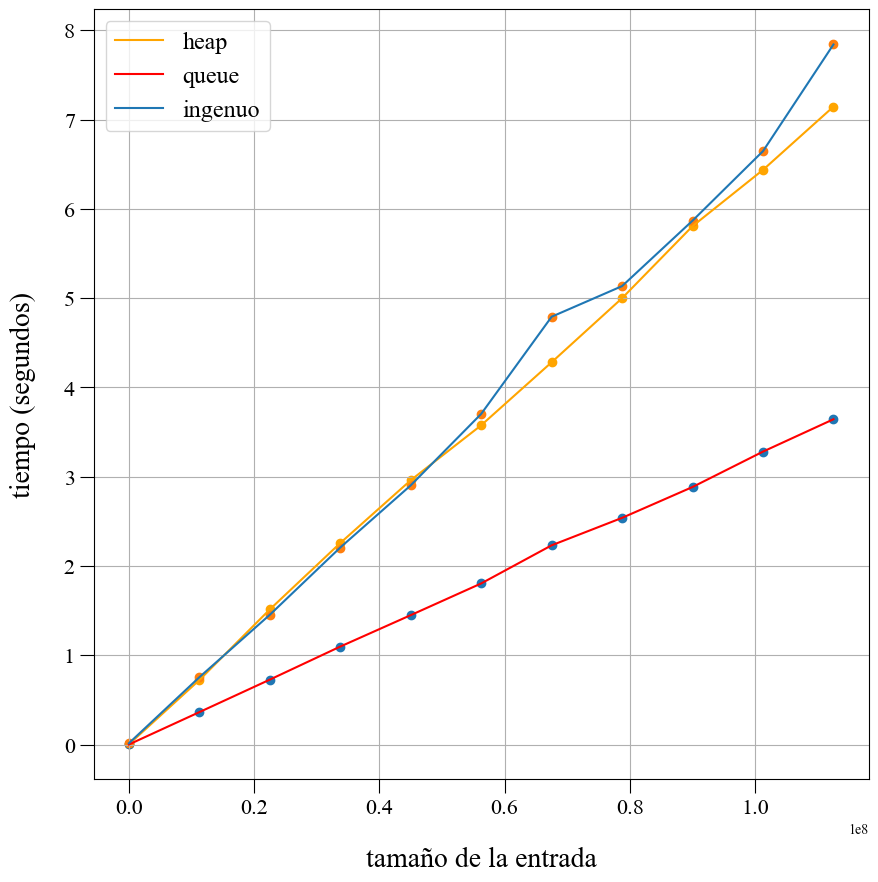
\includegraphics[scale=0.40, clip]{./files/src/.media/comparacion_triple.png}}

    \caption{Tiempo de ejecución de \textsc{tráfico} en función del tamaño de entrada $M$ para el algoritmo \textit{ingenuo}, el \textit{heap}, y \textit{queue}.}
    \label{grafico_1}
\end{figure}

La figura \ref{grafico_1} expone los resultados de la experimentación en grafos \textit{densos}. Nótese que a pesar de su superioridad asintótica, \textit{ingenuo} resulta el más lento, incluso en el último caso que ilustra un grafo completo. Quizás tiene constantes demasiado grandes. Claramente \textit{queue} es la más rápida, quizás por la eficiencia de la implementación de la estructura.

%\vspace{0.5em}
\begin{figure}[!htbp]
    \subfloat{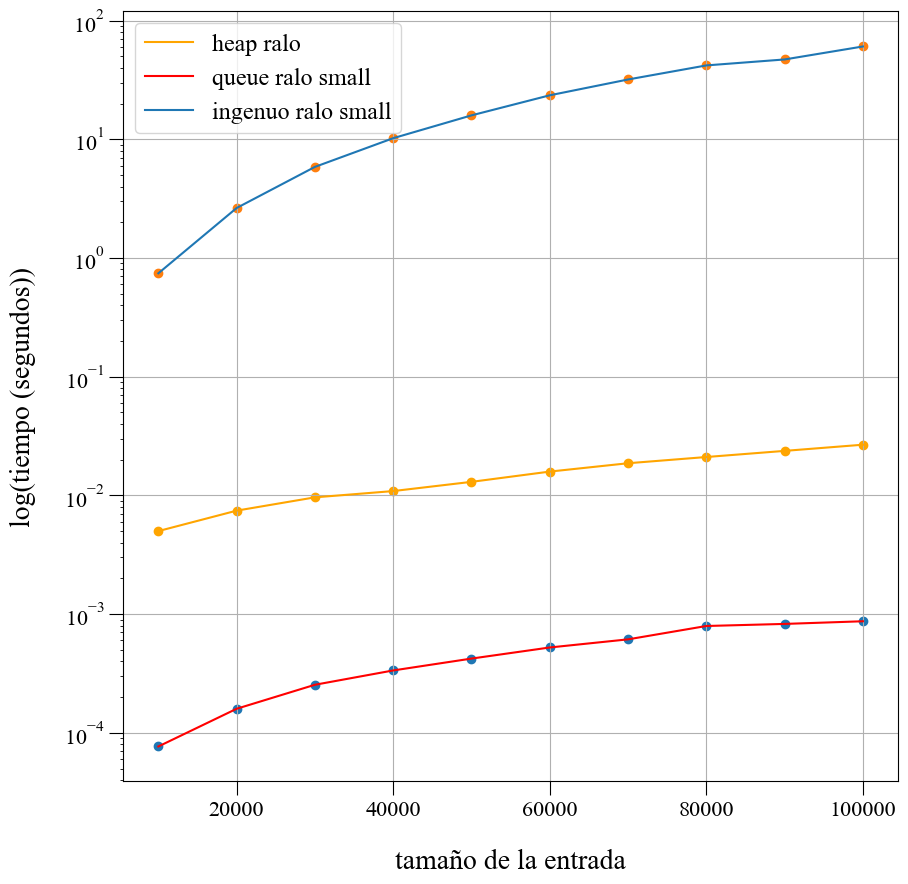
\includegraphics[scale=0.40, clip]{./files/src/.media/comparacion_rala_small.png}}
    %\hfill
    $\ \ \ \ $
    \subfloat{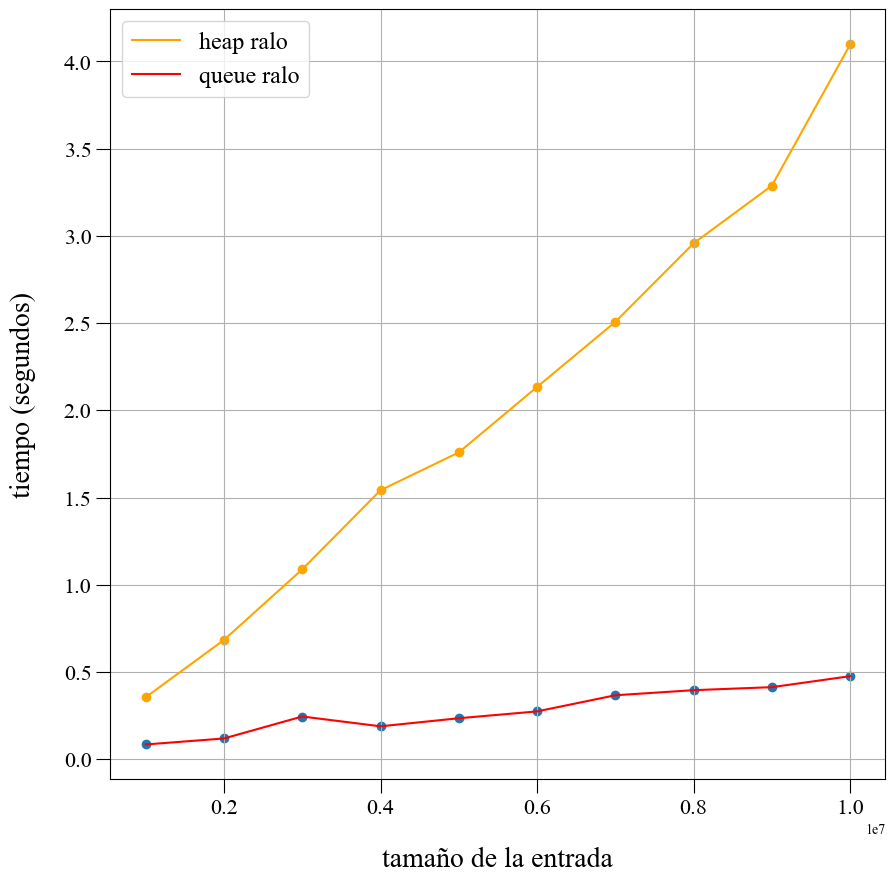
\includegraphics[scale=0.4, clip]{./files/src/.media/comparacion_rala_doble.png}}

    \caption{Izquierda: tiempo de ejecución de \textsc{trafico} en función del tamaño de entrada $N$ para el algoritmo \textit{ingenuo}, el \textit{heap}, y \textit{queue}. Derecha: ejecución de \textsc{tráfico} en función del tamaño de entrada $N$ con valores grandes, para \textit{heap} y \textit{queue}.}
    \label{grafico_2}
\end{figure}

La figura \ref{grafico_2} expone los resultados de las experimentaciones en grafos \textit{ralos}. Notese que el algoritmo \textit{ingenuo} resultó extremadamente ineficiente en esta situación, por lo que se debieron utilizar instancias pequeñas para poder compararlo con los otros algoritmos. Como los tiempos de \textit{heap} y \textit{queue} son demasiado bajos en esta instancia, se comparan los dos solos con una entrada 100 veces más grande. De vuelta se nota una clara diferencia a favor del algoritmo \textit{queue}.